
%(BEGIN_QUESTION)
% Copyright 2011, Tony R. Kuphaldt, released under the Creative Commons Attribution License (v 1.0)
% This means you may do almost anything with this work of mine, so long as you give me proper credit

A ``smart'' DP transmitter with built-in square root characterization is used to measure flow through a pipe.  The orifice plate range is 0 to 150 inches WC at 0 to 480 gallons per minute:

$$\includegraphics[width=15.5cm]{i03443x01.eps}$$

Operations personnel have strong reason to believe that the actual flow rate through this pipe is 160 GPM, yet the DCS registers a flow rate of 182.4 GPM.  Based on this information, determine the likely source of calibration error in this system.  Also determine whether this transmitter has square-root characterization enabled or not.

\vskip 10pt

Additionally, suggest a good ``next step'' to perform to either pinpoint the location of this problem or correct it.

\underbar{file i03443}
%(END_QUESTION)





%(BEGIN_ANSWER)

The calibration error lies either with the transmitter, the impulse lines (unequal fluid heights inside), or with the orifice plate itself.  The transmitter does have square-root characterization enabled.

\vskip 10pt

A good ``next step'' would be to block and equalize the transmitter manifold to check what its PV and AO parameters register with no applied differential pressure.

%(END_ANSWER)





%(BEGIN_NOTES)


%INDEX% Calibration, smart transmitter: digital trim
%INDEX% Fieldbus, HART: communicator variables
%INDEX% Measurement, flow: square root characterized pressure transmitter

%(END_NOTES)

